Packet analysis for each of the simulations was performed using the Wireshark
tool. This tool can be run on the PC running Mininet, and configured to monitor
the loopback address for OpenFlow packets, as described in the "Start Wireshark"
section here \cite{mininetWS}, or can be run on one of the Mininet host nodes.

\subsection{Denial of Service Results}

The Denial of Service network is initiated using the command show in Figure
\ref{fig:images-dosCli}. The output of running this command shows that all of
the required nodes and links are successfully created.

\begin{figure}[H]
	\centering
	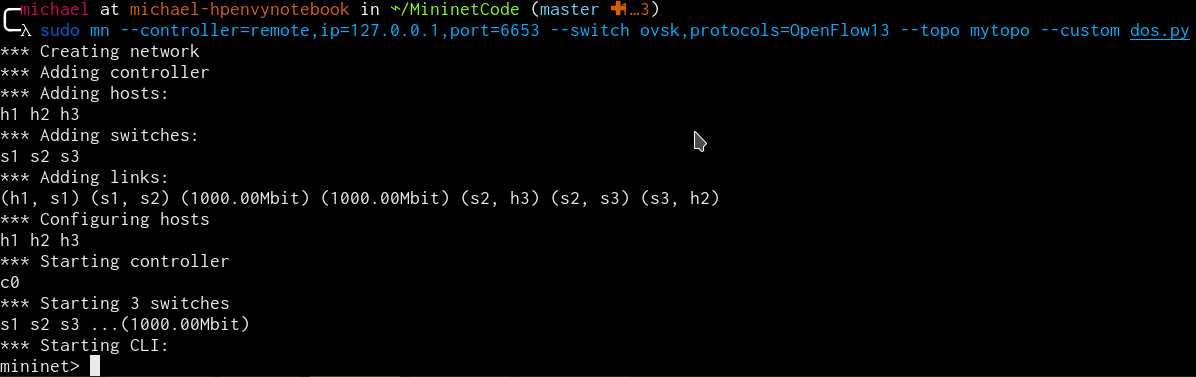
\includegraphics[width=0.8\textwidth]{images/dosMnCli}
	\caption{DoS Mininet CLI command output}
	\label{fig:images-dosMnCli}
\end{figure}

The Denial of Service topology was first verified within the Floodlight web
server. Figure \ref{fig:images-flDoS} displays the results of this:

\begin{figure}[H]
	\centering
	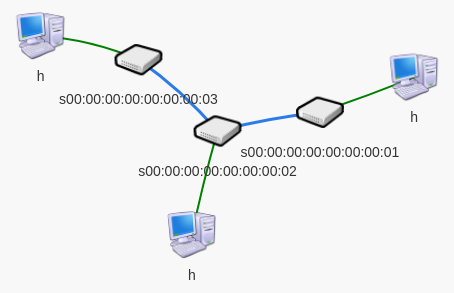
\includegraphics[width=0.8\textwidth]{images/flDoS}
	\caption{Denial of Service Floodlight Topology}
	\label{fig:images-flDoS}
\end{figure}

Once the network was deemed as correctly configure, the attack testing could
begin.

\subsubsection{SYN Flood}

The Wireshark packet analyzer tool is run on the attacking host. The filter
option used to capture only the outgoing SYN packets from the host is
'tcp.flag.syn== 1'. This results in the packet capture in Figure
\ref{fig:images-synFloodDosWs}. The set "SYN" flag can be seen in the packet
information in the bottom of the window.

\begin{figure}[H]
	\centering
	\includegraphics[width=0.8\textwidth]{images/synFloodDosWs}
	\caption{Denial of Service SYN Flood Captured Packets}
	\label{fig:images-synFloodDosWs}
\end{figure}

The SYN flood was initiated as discussed, using the hping command listed in
section 3.1.1. Once the flooding attack had been running for a period of time,
the ping command is used on the user host node, showing multiple timeouts,
indicating a denial of service has occurred.

\begin{figure}[H]
	\centering
	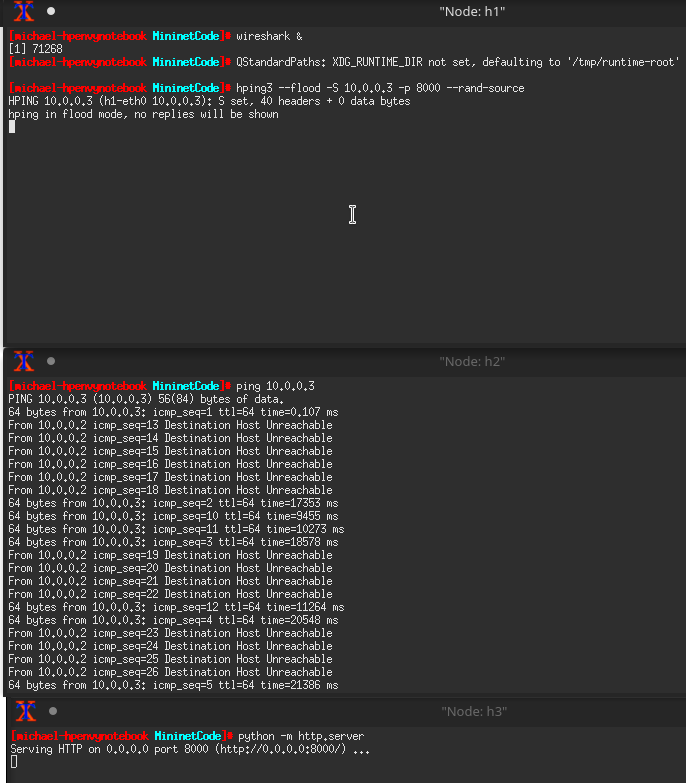
\includegraphics[width=0.8\textwidth]{images/synFloodResults}
	\caption{Terminal Output for the attacking node, target server, and user
	node}
	\label{fig:images-synFloodResults}
\end{figure}

The I/O graph output which can be viewed from the captured packets in Wireshark
shows the number of packets sent per second. There is a dip in the graph where
the number of sent packets drops to zero, which could account for the successful
ping connections from the user node.

\begin{figure}[H]
	\centering
	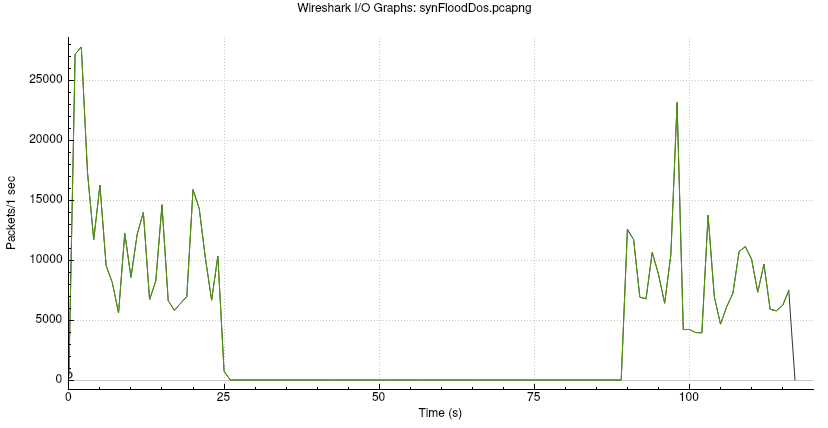
\includegraphics[width=0.8\textwidth]{images/synFloodDosIOGraph}
	\caption{Denial of Service SYN Attack I/O Graph}
	\label{fig:images-synFloodDosIOGraph}
\end{figure}

\subsubsection{ICMP Flood}

The Wireshark packet analyzer tool is run on the attacking host. The filter
option used to capture only the outgoing SYN packets from the host is
'icmp'. This results in the packet capture in Figure
\ref{fig:images-icmpFloodDosWs}. The set "SYN" flag can be seen in the packet
information in the bottom of the window.

\begin{figure}[H]
	\centering
	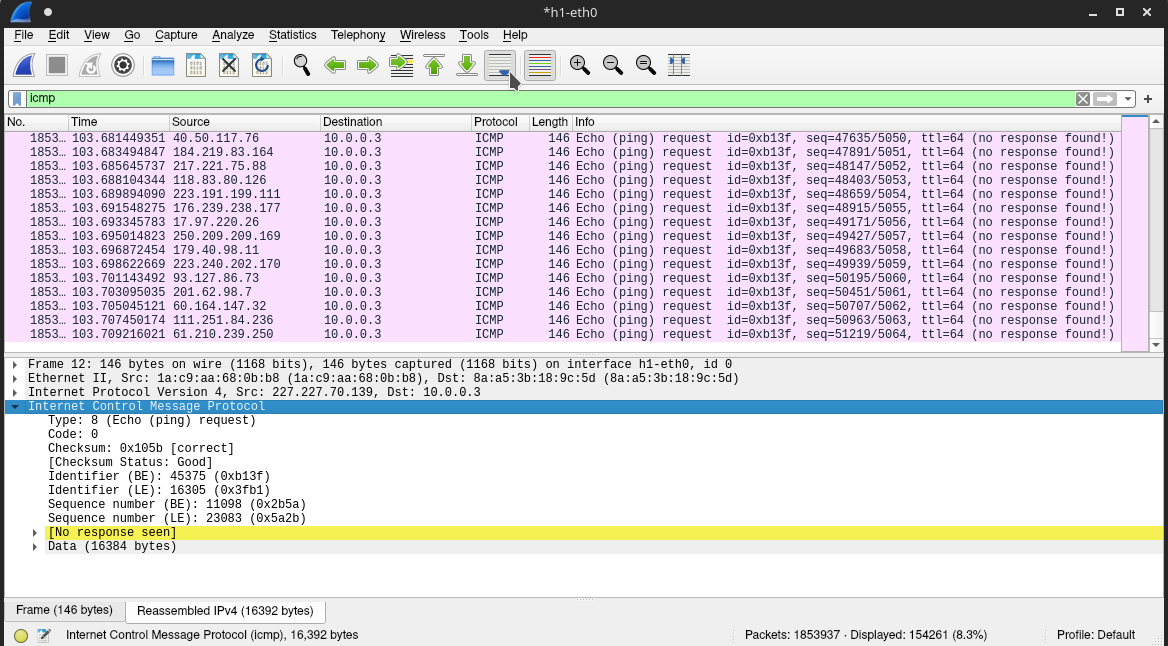
\includegraphics[width=0.8\textwidth]{images/icmpFloodDoSWs}
	\caption{Denial of Service ICMP Flood Captured Packets}
	\label{fig:images-icmpFloodDosWs}
\end{figure}

The SYN flood was initiated as discussed, using the hping command listed in
section 3.1.2. Once the flooding attack had been running for a period of time,
the ping command is used on the user host node, showing 100\% packet loss,
indicating a denial of service has occurred.

\begin{figure}[H]
	\centering
	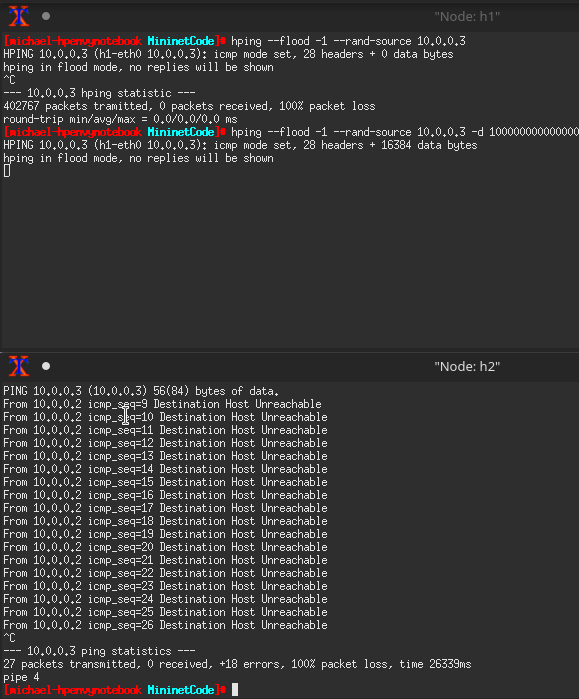
\includegraphics[width=0.8\textwidth]{images/IcmpFloodDosCli}
	\caption{Denial of Service ICMP Flood Output}
	\label{fig:images-icmpFloodDosCli}
\end{figure}

The I/O graph output which can be viewed from the captured packets in Wireshark
shows the number of packets sent per second. There are a number of dips in the
graph where the number of sent packets drops, at some points to zero, however,
this did not result in a successful ICMP echo response from the server.

\begin{figure}[H]
	\centering
	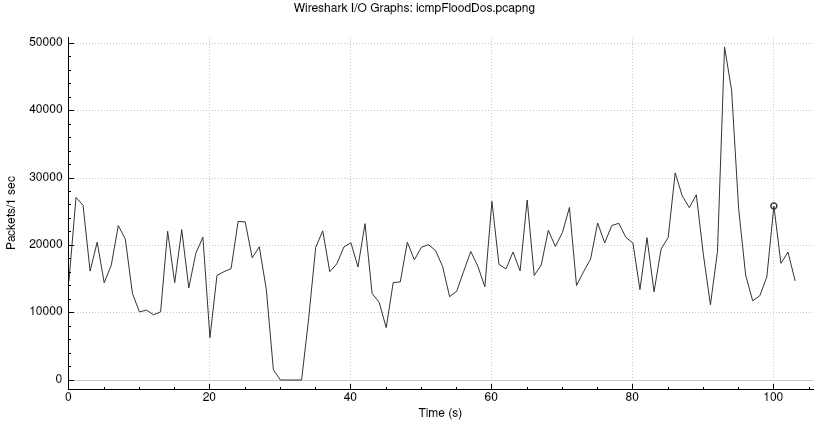
\includegraphics[width=0.8\textwidth]{images/icmpFloodDos}
	\caption{Denial of Service ICMP Attack I/O Graph}
	\label{fig:images-icmpFloodDosIOGraph}
\end{figure}

\subsubsection{Mitigation}

In order to utilise the benefits of SDN and the Floodlight controller, both of
these attacks could be mitigated using Network Access Control Lists. NACLs allow
for the blacklisting or whitelisting of different IP addresses for certain
protocols. For example, ICMP can be disabled for all nodes by specifying a deny
rule for the CIDR rage 0.0.0.0/0. In the case of the SYN Flood, which uses
random source IP addresses, whitelisting could be used to allow traffic from
nodes within the network, such as the user node, or for the case of the ICMP
Flood, which does not use spoofed IP addresses, the attack source IP address can
be blacklisted, as shown in Figure \ref{fig:images-icmpDosAcl}.

\begin{figure}[H]
	\centering
	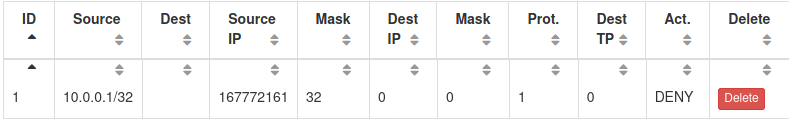
\includegraphics[width=0.8\textwidth]{images/icmpDosAcl}
	\caption{NACL Rule to deny ICMP from an attacking node}
	\label{fig:images-icmpDosAcl}
\end{figure}

The mitigating effects of this ACL can be seen in Figure \ref{},

\subsection{Distributed Denial of Service}

The Distributed Denial of Service topology was verified within the Floodlight
web server. Figure \ref{fig:images-flDDoS} displays the results of this, with
8 switches with 8 hosts each, and a final switch connected to the single target
server node.

\begin{figure}[H]
	\centering
	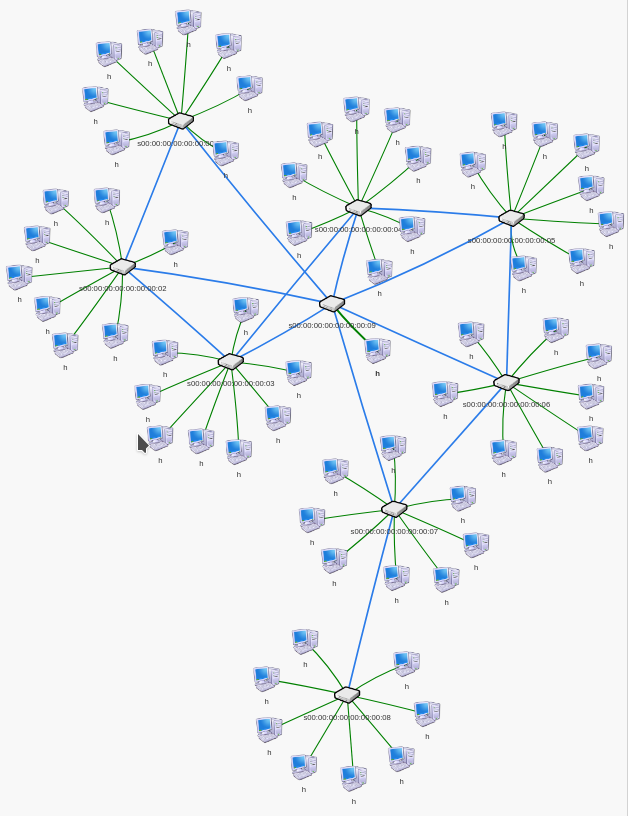
\includegraphics[width=0.8\textwidth]{images/flDDoS}
	\caption{Distributed Denial of Service Floodlight Topology}
	\label{fig:images-flDDoS}
\end{figure}

\subsubsection{SYN Flood}


\subsubsection{ICMP Flood}
